\chapter{Introduction}
\section{Motivation}
% 建立投资组合,不仅需要时间序列上的不相关性,也需要经济上潜在的不相关性。edge的weight代表价格时间序列上的不相关性,而方向代表经济上的。从而对建立有效的投资组合提供建议。
Financial markets are complex systems, the interconnectedness and interdependencies of industrial sectors in the economy are highly inter-coupled with strong correlations with stock price fluctuations, i.e., the price returns of each coupling stocks underlying certain economic link, e.g. two companies that manufacture similar products, or both in one supply chain. Such behaviours can hardly be explained by traditional financial models and theories.

During recent times, weighted but undirected complex network models have been applied to study the correlations of stock prices. Prevailing approach is to use companies as nodes, and correlations between each pair of stock price time series, return time series, or fluctuation patterns as links. As a result, much of the previous researches have proved the represented complex networks of worldwide stock markets are scale-free and small-world~\cite{cnsm, perspective}. However in theory, directed complex networks for the stock market can be achieved hence more potential information can be produced which is helpful for investment decisions and financial market supervisions.

For building an investment portfolio of stocks, one should consider not only about the irrelevancy on price or price return time series, but also about the irrelevancy on economical activities between firms and industries. Naturally and instinctively, we can depict the interactions of economical activities between stock-pairs as the directions of edges in the stock complex network, and the weights of the edges are still determined by the correlations of stock price return time series as many previous researches practised. Therefore, some guidance may be offered for investors to build more effective portfolio and market supervisors to avoid potential crisis according to the study of directed stock complex network.

% hence a new perspective is needed

The goal of this thesis is to reveal the interactions of economical activities between companies and utilise them into the topological analysis and visualisation of constructed directed complex networks as so far no previous work has attempted to construct a directed network about stock markets. In addition, suggestions for stock market are provided according to the results and findings.

In addition to this approach, there was a goal of using machine learning techniques to predict the directions of stock complex network. However, these results were not as successful and conclusive as we expected. They are reported in the last chapter of this thesis as additional work complementing the core analysis of this thesis based on complex network theory.

% In the viewpoint of directed networks, the analysis of stock complex network can provide new 

\section{Objectives and deliverables}
The goal of this thesis is to construct a directed complex network using economical industrial transaction data and stock price data to depict the US stock market by means of topological properties analysis, community detection and visualisation. Same-sized directed Watt-Strogats small-world network and random networks are generated for the purpose of comparison. This thesis will explore whether the conclusions are consistent with the undirected complex network researches.

\vline

Objectives produced:

\begin{itemize}
	\item To normalise the Economic Input-Output (EIO) tables into matrices for setting thresholds.
	\item To generate a matrix of correlation coefficients for all stock-pairs.
	\item To set appropriate thresholds of correlation coefficient and normalised economical transactions.
	\item To construct directed-unweighted and directed-weighted stock price return networks.
	\item To study the topological properties of directed stock price return networks.
	\item To detect communities in the directed stock price return networks.
	\item To visualise the directed stock price return networks.
	\item To study the relationships between price return and betweenness centrality.
\end{itemize}

\vline

Deliverables produced:

\begin{itemize}
	\item Stock counts by industries.
	\item Matrix of EIO transaction flows.
	\item Heatmap of combinations of thresholds of directed demands and directed requirements flows and correlation coefficients.
	\item Two benchmarking networks: directed Watts-Strogatz (WS) small-world network and directed Erdős–Rényi (ER) random network.
	\item Directed-unweighted and directed-weighted stock network.
	\item Topological properties of studied networks.
	\item Community partition of directed-unweighted stock network.
	\item We plan to produce a research thesis to submit to a journal. We are thinking of journals like:  \textit{Physica A, Journal of Mathematical Finance, Journal of Applied Mathematical Finance, Applied Network Science}.
\end{itemize}

\section{Proposed methodology}
% summary and put a diagram of the part of my thesis
\begin{figure}
	\begin{center}
		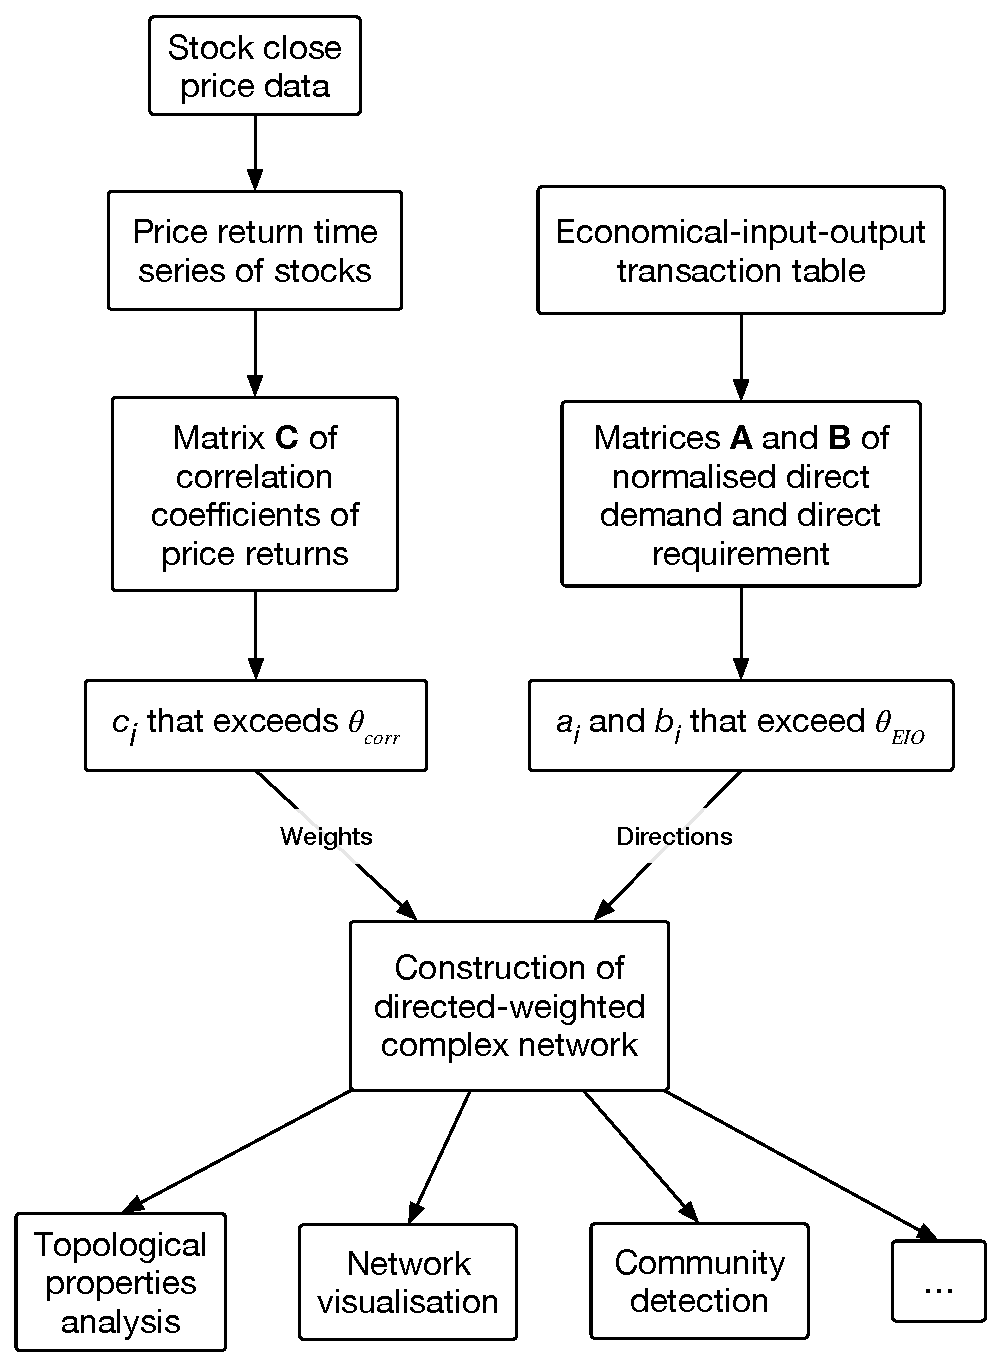
\includegraphics[width=11cm]{methodology_diagram}
	\end{center}
	\caption{The methodology}
	\label{fig:methodology_diagram}
\end{figure}

In this thesis we proposed a method to generate directed-unweighted complex network and directed-weighted complex network for stock market, especially for the US stock market in the year of 2016. Analysis of topological properties and comparison with benchmarking networks provide unique insights towards its continuity or uncontinuity features to conventional undirected stock networks in previous researches and its compositional structure.

\section{Summary of results}
While working on this thesis, the following achievements have been made that will be described in detail in this thesis:

\begin{itemize}
	\item To calculate topological property values to study the the properties of stock complex networks.
	\item To compare the directed-unweighted stock complex network with generated directed WS small-world network and directed ER random network.
	\item To apply community detection algorithm to find possible communities of the directed-unweighted stock complex network.
	\item To generate bivariate distributions between betweenness centralities and functions of stock daily return to find the potential relationships between them.
\end{itemize}

\section{Outline of the thesis}
The rest of this thesis is organised as follows. Chapter~\ref{cpt:back} discusses the development of quantified financial analysis for stock markets and the application of complex theories of complex networks towards stock markets. The subsequent chapters of methodologies introduce the critical analytical methods implemented in the research by this thesis. Detailed outcomes are then illustrated in chapter~\ref{cpt:result}. Other results about the method of using machine learning techniques to help construct directed stock networks are presented in chapter~\ref{cpt:other}. Finally, the findings and conclusions are discussed in chapter~\ref{cpt:conclude}.
